%% This file is to be used as a template for your submission. 
%% Rename this file and replace the text with the text of 
%% your manuscript.
%%
%% The standard LaTeX document class "article" is recommended. 
%% Use options letterpaper and 12pt.
\documentclass[letterpaper,12pt]{article}

%% This is the recommended preamble for your document.

%% Load De Gruyter specific settings 
\usepackage{dgjournal}          

%% The mathptmx package is recommended for Times compatible math symbols.
%% Use mtpro2 or mathtime instead of mathptmx if you have the commercially
%% available MathTime fonts.
%% Other options are txfonts (free) or belleek (free) or TM-Math (commercial)
\usepackage{mathptmx}

% Big maths font
%\everymath{\displaystyle}
\everymath=\expandafter{\the\everymath\displaystyle}

%% Use the graphics package to include figures
\usepackage{graphicx}
\usepackage{float}

%% Use natbib with these recommended options
\usepackage[authoryear,comma,longnamesfirst,sectionbib]{natbib} 
\usepackage{url}

% Centre table cells with custom width, e.g. C{2cm}
\usepackage{array}
\newcolumntype{C}[1]{>{\centering\let\newline\\\arraybackslash\hspace{0pt}}m{#1}}

%% Start your document body here
\begin{document}

%% Do NOT include any fronmatter information; including the title, author names,
%% institutes, acknowledgments and title footnotes (author information, funding
%% sources, etc.). Start the document with the first section or paragraph of
%% the article.

\section{Introduction}

\subsection{The Tennis Betting Industry}

Tennis is one of the world's most popular individual sports and thus is also one of the most heavily traded on betting exchanges.  The market continues to grow at a remarkable pace; for example, during the Wimbledon 2006 final between Roger Federer and Rafael Nadal, Betfair processed approximately \pounds25 million worth of matched trades.  In comparison, the Wimbledon 2012 men's final between Andy Murray and Roger Federer matched almost \pounds56 million worth of bets.  Such interest is not limited to Grand Slam finals either; during the women's semi-final of the Sony Ericsson Open 2011 between Maria Sharapova and Andrea Petkovic, \pounds10 million was traded on Betfair\footnote{http://www.fracsoft.com}.

Tennis is well suited to in-play trading on exchanges since points are played at a steady rate, are clearly separated, and are consistently won and lost by both participants, leading to frequent (and often dramatic) changes in fortune for players but at relatively predictable intervals.  Consequently, the odds can very quickly swing back and forth as traders react to on-court events, generating potential money-making opportunities.  This, in combination with the fact that tennis markets have the ability to offer only a few outcomes (e.g.\ in a Match Odds market, there are only two outcomes, either one player wins or the other does), ensures its popularity.  Around 80\% of money waged on tennis matches is bet while the match is in progress\footnote{http://www.sportspromedia.com/guest\_blog/peter\_webb\_why\_tennis\_is\_big\_business\_for\_bookmakers}.

Tennis also happens to be a relatively simple game to model in comparison with other highly complex sports such as football or cricket.  It is just a series of discrete repeated contests, i.e. points, and calculations essentially boil down to the probability each player has of winning a given point.  The scoring system has a fixed number of hierarchical states; points are nested within games, games within sets, and sets make up a match.

\subsection{Player Retirement in Professional Tennis}

In professional tennis, a player may `retire hurt' from a match at any time should they feel they are unable to complete the match due to injury or illness, or that it is unwise to continue in case they aggravate their condition.  The match is consequently awarded to the opponent regardless of the current match state.  A \textit{walkover} occurs when a player withdraws from a match before it has begun.  In-play injuries are common occurrences in tennis as a whole.  Between 2000 and 2009, there was a retirement during approximately 3.9\% of Grand Slam men's singles matches\footnote{http://www.tennis.ukf.net/stats15.htm}.  Betting companies take different approaches when dealing with the issue of player retirement.  Typically, they fall into one of four categories (with regards to Match Odds markets)\footnote{http://rebelbetting.com/faq/tennis-rules}:

\begin{description}
	\item[Category 1: Ball-Served Rule] For a bet to stand, at least one ball must have been served, e.g. Ladbrokes.
	\item[Category 2: One-Set Rule] For a bet to stand, at least one set must have been completed in the match.  However, if a player retires from the match before the first set is over, all bets are cancelled and stakes are refunded, e.g. Betfair.
	\item[Category 3: Two-Sets Rule] For a bet to stand, at least two sets must have been completed in the match, e.g. TheGreek.
	\item[Category 4: Match-Completed Rule] The entire match must be completed for a bet to stand, e.g. Paddy Power.
\end{description}

Markets offered on the outcomes of individual games or sets are always rendered void unless the result has been unconditionally determined.  UK-based Betfair, the world's first betting exchange, falls into \textit{Category 2} of the tennis betting retirement payout policies with respect to its in-play Match Odds market.  Betfair's Set Betting market is always voided in the event of a retirement since if the match is not finished, we do not have a final score.

\subsection{Premise}

Figure \ref{djokovicnadal} displays the evolution of implied match-winning probabilities for Novak Djokovic when he played Rafael Nadal in the US Open 2011 Men's Final.  The blue line shows implied probabilities extracted from the Betfair Set Betting market, the red line shows implied probabilities extracted from the Betfair Match Odds market, and the green line shows the positive difference of the Set Betting probability minus the Match Odds probability.  As you can see, both markets are closely matched.  This is intuitive since the probability of Djokovic winning the match should be the same as the sum of the probabilities of the final score being 3-0, 3-1, or 3-2 in Djokovic's favour.  This is especially true in high profile matches such as this one where the markets are very liquid and millions of pounds are being traded in both, leading them to produce very accurate odds.

\begin{figure}[H]
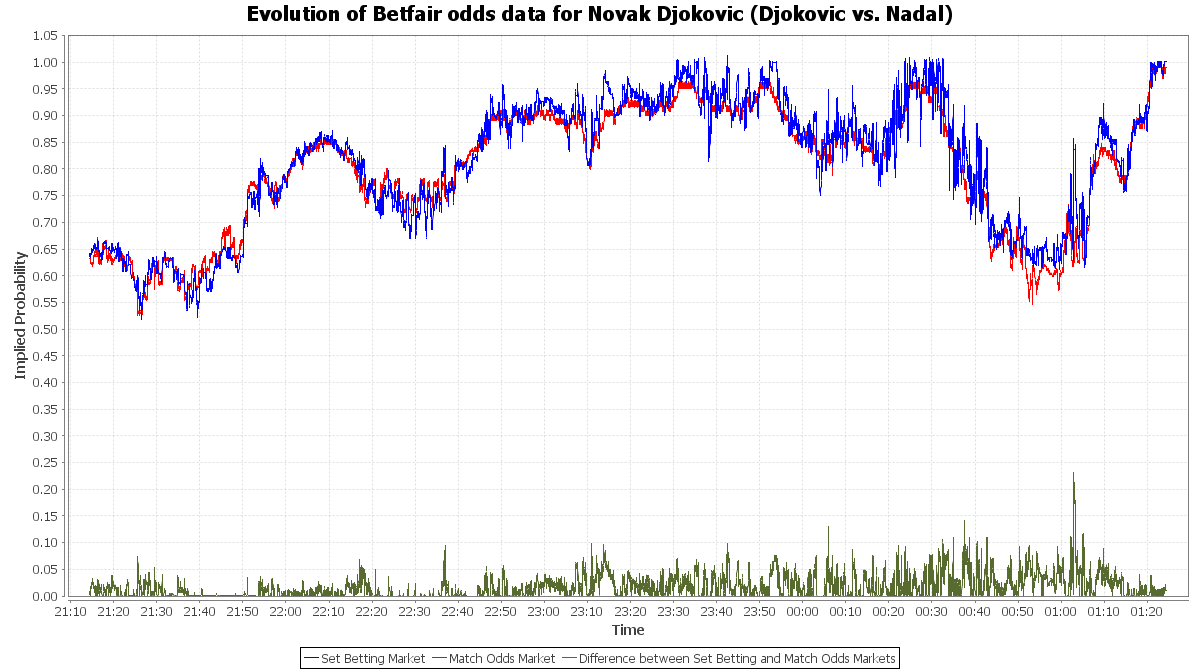
\includegraphics[width=12.5cm]{matches/djokovicnadal}
\centering
\caption{Evolution of implied match-winning probabilities extracted from the Betfair Match and Set Betting markets as well as the gap between them for Novak Djokovic - \textit{Djokovic vs. Nadal (US Open 2011 Men's Final)}}
\label{djokovicnadal}
\end{figure}

Compare with Figure \ref{murrayberrer} which displays the evolution of implied match-winning probabilities for Andy Murray when he played Michael Berrer in the French Open 2011 Men's Third Round.  In particular, observe where the Match Odds probability of Murray winning the match suddenly drops \textit{almost 60\%}.  This phenomenon in the odds data occurred during a \textit{single point in the match}.  Although there are a few anomalous events which could have led to this huge and rapid swing in the market such as a disqualification, the evidence here weighs heavily towards the \textit{injury} that was suffered by Andy Murray.  We quote from the \textit{BBC Sport}\footnote{http://www.bbc.co.uk/sport} live text commentary of the match during this point:

\begin{itemize}
	\item ``Big, big trouble for Andy Murray, who has gone over on his right ankle and looks in real pain. Not sure whether he will be able to continue. Unbelievable.''
	\item ``We are going to have a medical time-out while Murray has treatment. He slipped as he ran in to put away a forehand, and the replays are not very pleasant to watch.''
\end{itemize}

In this case, the injury did not cause Murray to retire from the match and he went on to win in straight sets, as reflected in the subsequent recovery of his odds to win.  Nevertheless, it is clear the market reacted to this event and its opinion on Murray's chances of winning the match was severely affected.

\begin{figure}[h!]
  \centering 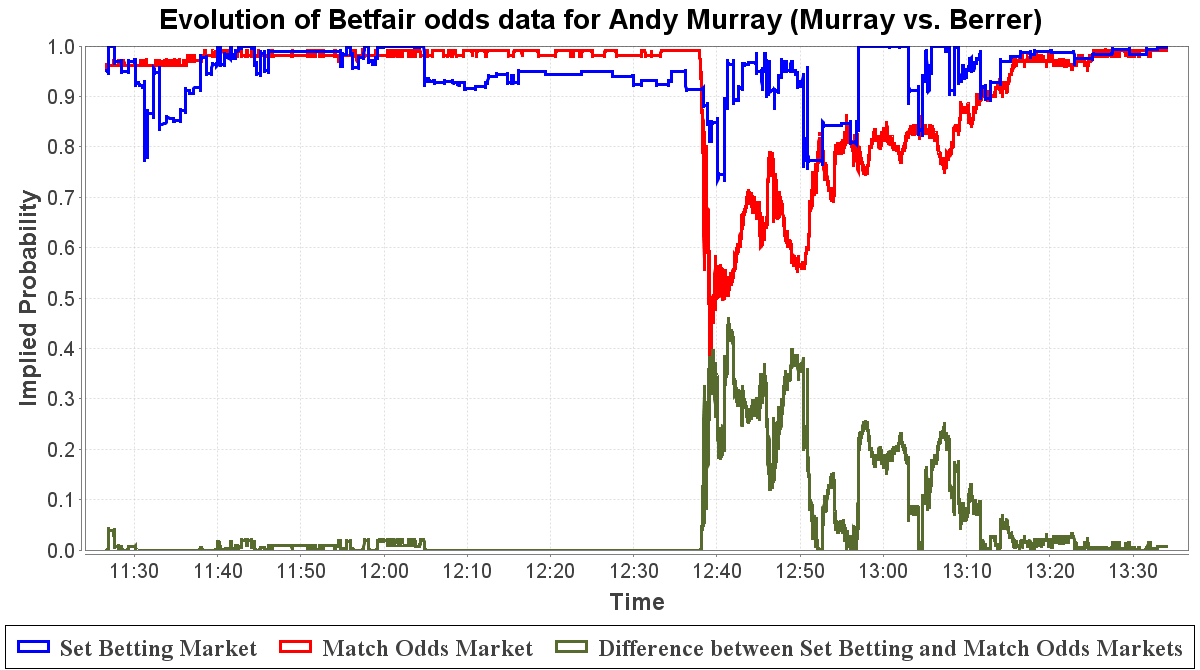
\includegraphics[width=12.5cm]{matches/murrayberrer}
  \caption{Evolution of implied match-winning probabilities extracted from the Betfair Match and Set Betting markets as well as the gap between them for Andy Murray - \textit{Murray vs. Berrer (French Open 2011 Men's Third Round)}}
  \label{murrayberrer}
\end{figure}

We can observe the evolution of the Betfair Set Betting and Match Odds markets in order to help us \textit{quantify} a player's risk of retirement.  For example, we can see from the Murray vs Berrer match when the injury occurred that the Match Odds implied probability dropped sharply but the Set Betting implied probability remained relatively stable.  If a player becomes injured and concedes the match at any point, traditional bookmakers will usually cancel bets in all markets (they fall into Category 4).  Betfair will refund money on final score bets (Set Betting) but will still pay out on bets to win (Match Odds) as long as at least one set has been played (since the match has a winner but no final score).  In this way, the Betfair Set Betting market \textit{simulates} a Match Odds market that \textbf{ignores risk of retirement} whereas the actual Betfair Match Odds market \textbf{takes into account retirement risk}, given one set has been played.  Consequently, we see discrepancies between the match and final score odds in such scenarios (possibly more so beyond the first set) as we do in the Murray match.  
The theory is that the probability of a player retiring \textit{at some point during the remainder of the match} should be somehow encapsulated within the difference between the two markets, i.e. the combined opinions of all the traders betting in those markets (the wisdom of the crowd).  All the complex factors which lead to a player deciding to retire such as the state of the match, the seriousness of the injury, the importance of the match, even their past history of retirements, should be \textit{some function} of this gap in the odds.

\section{Background}

\subsection{The Physical Demands of Professional Tennis}

Various papers have been written on tennis-related injuries from a physiological perspective.  In particular, \cite{demands} attempted to quantify the demands in professional male tennis by analysing the number and type of strokes played per game for 22 players from three Grand Slams.  They found that the serve was the predominant stroke played in service games (up to 60\%) whereas topspin forehands and backhands were more frequent when receiving.  The 2003 US Open winner hit over 1000 serves during his seven matches at the tournament.  More strokes are played at the French Open than Wimbledon due to the relative speeds of the clay and grass court surfaces leading to longer rallies at Roland Garros.  Importantly, Johnson and McHugh discuss the strain that playing a point inflicts on the body.  They report that over 50\% of world-class tennis players experience shoulder discomfort during their career and 80\% of these cases stem from overuse.  Stroke production in tennis involves generating repetitive forces and motions that are of high intensity and short duration.  For example, the serve is the most strenuous stroke on the upper extremity with internal rotation velocities of the humerus reaching 2420 degrees per second for elite players during the acceleration phase.  This, coupled with the relentless demands the ATP (Association of Tennis Professionals) and WTA (Women's Tennis Association) tours place on players, suggest that it is no surprise injuries are an issue in the world of professional tennis.

\subsection{Existing Tennis Models}

There have been many past works on the topic of modelling tennis.  \cite{omalley} presents what are considered the \textit{tennis formulae}.  The tennis formulae are a hierarchical series of equations that compute the probability a given player will win a tennis match given the probabilities that the given player and his/her opponent will win any of their service points.  Combined together are individual formulae for the probabilities of winning games, sets, and tiebreaks.

\cite{servefirst} more comprehensively explore the use of recurrence relations to model tennis, utilising them to calculate probabilities of winning tournaments and also proving explicitly that the probability of winning a set or match does not depend on which player serves first.  \cite{excel} experiment with the same idea in Microsoft Excel.  They investigate using six parameters rather than just the two point-winning probabilities taking into account service faults.  Consequently, for each player they input the probability of a successful first serve, the probability of winning a point on first serve, and the probability of winning a point on second serve.  \cite{willyk} also designed a low-level model of tennis points, taking into account such events as service faults and service aces, in order to predict the outcome of matches.  They tailor their input probabilities to the specific returning capabilities of the given opponent (not an average player), estimated using historical statistics.  They find that their model was able to successfully predict 67\% of outcomes from a sample of 1839 ATP matches played during 2011.  Since we are already adding further complexity with the probability of retirement, we shall concentrate on extending a simpler, two parameter version of a tennis model.  \cite{momentum} continued with an investigation into player momentum in tennis matches by slightly perturbing point-winning probability depending on how much the given player is leading or trailing the match by (essentially introducing a dependency between points).

The vital thing to note is that no previous tennis model incorporates retirement risk as a factor.  They are therefore unable to account for the evolution of odds in in-play betting markets that utilise different retirement payout policies.

\newpage

\section{A Model for Retirement Risk}

\subsection{Definition}

The granularity of the model is point-level as this is compatible with the structure of standard tennis models.  When a tennis player plays a point, he or she potentially puts great strain on their body.  This strain naturally leads to a chance of an injury occurring.  For the vast majority of points played, the strain is perfectly manageable and does not lead to injury.  For example, Grand Slam winners can hit over 1000 serves during the course of the tournament without issue.  Occasionally however, the body fails to cope with the strain, or the strain is for some reason much more acute than normal (e.g.\ remember Andy Murray twisting his ankle), and an injury occurs.  When a player does get injured during a match, it does not always end in retirement.  Players often soldier on at least for a few points and may even recover from the injury as the match progresses.  
Using this intuition, we present an elegant model for the probability a player will retire \textit{on a given point} in a tennis match:

\begin{center}
\begin{eqnarray*}
r_0 &=& 0 \\
r_{n+1} &=& min(\rho r_n + XY, 1) \\
\end{eqnarray*}
\end{center}

where $r_n$ is the given player's risk of retirement on point $n$ of the match, $0 \leq \rho \leq 1$, and $X$ and $Y$ are random variables.  Do not confuse $r_n$ with what we are hoping to eventually calculate which is $R_n$, the risk of retiring at some point during the remainder of the match from point $n$.  We say that players start a match with zero probability of retiring ($r_0 = 0$), although in principle it is possible players might start a match with a niggling injury, in which case the magnitude could be inferred from observations of two or more match markets with differing retirement policies.  When setting $r_{n+1}$, we make sure to take the minimum of the calculated $r_{n+1}$ and 1, since retirement risk is a probability and cannot be greater than 1.  The Bernoulli random variable, $X$, with success parameter $c$, models the chance of an injury occurring on a given point.  The random variable, $Y$, models the magnitude of an injury should it occur and is truncated exponentially distributed with rate parameter $\lambda$ and upper bound 1, i.e. minor bumps and bruises are more common than serious, match-ending injuries.  The decay parameter, $\rho$, models the idea that players recover from injuries as matches progress.  For the purpose of avoiding too complex a model, we make the simplifying assumption that $\rho$ and the distributions of $X$ and $Y$ are the same for both players.

We incorporate our model of retirement risk into a \textit{tennis match simulator} capable of approximating match-winning probabilities.  We input the point-winning probability for each player as well as the current score and current point-level retirement risks, and simulate a large number of matches using the same parameters for each match.  The simulator is probabilistic but we expect convergence towards exact match-winning probabilities.  The greater the number of \textit{runs} (i.e. matches played), the greater the accuracy of the approximation generated by the simulator.  The proportion of matches the modelled player wins out of the total number of runs is an estimation of the chance of winning.  Similarly, the proportion of matches the modelled player retires from out of the total number of runs is an estimation of the risk of retiring.

A given point in a simulated match has four possible outcomes.  Either player can win the point or either player can retire from the match.  To resolve a point, we generate a random number between 0 and 1 and observe which of the bins (as shown in Figure \ref{bins}) the number falls in.  The match ends if it falls in one of the retirement bins (which is why $r_A$ and $r_B$ are usually 0 else you will rarely be able to get through even a single match without retiring), otherwise one of the players wins the point ($P_A$ is the point-winning probability on serve of Player A) and the match continues (unless it was their match point).

\begin{figure}[H]\Large
	\begin{center}
		\begin{tabular}{|C{3.5cm}|C{2.5cm}|C{0.7cm}|C{0.7cm}|}
			\multicolumn{1}{l}{\small{0}} & \multicolumn{1}{r}{} & \multicolumn{1}{r}{} & \multicolumn{1}{r}{\small{1}} \\
			\hline
			$P_A$ & $1 - P_A$ & $r_A$ & $r_B$ \\ \hline
		\end{tabular}
	\end{center}
	\caption{The four possible outcomes of a point in our modified tennis match simulator where Player A is serving}
	\label{bins}
\end{figure}

To imitate the Betfair Set Betting market (or equivalently, a Match Odds market using a Paddy Power-style \textit{match-completed} payout policy), we can use O'Malley's tennis formulae which ignore retirement risk (the \textit{No Retirement Risk} column in Figure \ref{outcomes}).  We use our tennis match simulator to imitate a Match Odds market as it might behave using the different retirement betting payout policies by calculating the remaining probabilities in the right-most three columns.

\begin{figure}[H]
	\begin{center}
	\renewcommand{\arraystretch}{1.8}
		\begin{tabular}{|C{1.2cm}|C{1.4cm}|C{2.8cm}|C{2.4cm}|C{2.4cm}|}
			\hline
			\textbf{Player} & \textbf{No Ret. Risk} & \textbf{Normal Win With Ret. Risk} & \textbf{Retirement in 1st set} & \textbf{Retirement after 1st Set} \\ \hline
			$A$ & $W_A$ & $W'_A$ & $R'_A$ & $R^{''}_A$ \\ \hline
			$B$ & $W_B$ & $W'_B$ & $R'_B$ & $R^{''}_B$ \\ \hline
		\end{tabular}
	\renewcommand{\arraystretch}{1}
	\end{center}
	\caption{Probabilities that can be closely approximated by our modified tennis match simulator}
	\label{outcomes}
\end{figure}

$W'_A$, for example, is the probability of Player A winning the match normally by achieving 3 sets and not via Player B retiring.  Note that we can (re-)calculate the match-winning probability for Player A ignoring retirement risk ($W_A$) as a sanity check by computing:

\begin{center}
	$\frac{W'_A}{W'_A + W'_B}$
\end{center}

In addition, the ratio of $W_A$ to $W_B$ is the same as the ratio of $W'_A$ to $W'_B$.  This is because we assume that the point-winning probabilities of each player are unaffected by injury.  We can imitate a Betfair-style \textit{after one set} payout policy market for Player A by computing:

\begin{center}
	$\frac{(W'_A + R^{''}_B)}{(W'_A + R^{''}_B) + (W'_B + R^{''}_A)}$
\end{center}

which is the probability that Player A wins normally plus the probability that Player B retires after the first set, normalised by the sum of the probabilities that either player wins the match normally and either player retires after the first set.  Similarly, we can imitate a Ladbrokes-style \textit{after one ball} payout policy market for Player A by computing:

\begin{center}
	$\frac{(W'_A + R_B)}{(W'_A + R_B) + (W'_B + R_A)}$
\end{center}

where $R_A = R'_A + R^{''}_A$ and $R_B = R'_B + R^{''}_B$.  This is essentially a re-calculation of the \textit{Normal Win With Retirement Risk} column.

\subsection{Simulated Results}

We have introduced three unknowns into our simulator; $c$ is the success parameter of the Bernoulli distribution (per point injury probability) corresponding to random variable $X$, $\lambda$ is the rate parameter of the injury magnitude truncated exponential distribution corresponding to random variable $Y$, and $\rho$ is the injury recovery factor.

Figure \ref{variabletable} displays a table describing the majority of the variables we have introduced thus far.  An appropriate parameterisation of the model would be values for the unknown input variables, $c$, $\lambda$, and $\rho$, that generate $R_A \approx R_B \approx 1.95\%$ when input into our modified simulator at the start of a 5-set match.  We believe these match-level retirement risks are justified as it corresponds to the 3.9\% chance of such a match ending in retirement as seen in men's Grand Slam singles matches between 2000 and 2009.  Given \cite{dominance} find that the average point-winning probability on serve for a top-level professional tennis player is 0.645 for men and 0.560 for women, we choose 0.6 as a reasonable value for $P_A$ and $P_B$ which denotes an even match.  The goal now is to \textit{fit} the model by adjusting the parameter values to accurately reflect real-world events.

It is possible to use a multivariate direct-search optimisation algorithm such as the Nelder-Mead simplex method (an algorithm primarily designed for statistical parameter estimation problems such as ours) to approximate a set of values for these parameters.  Specifically, we used a constrained version of the Nelder-Mead algorithm in order to ensure logical bounds $0 < c, \rho < 1$ and $\lambda > 0$.

\begin{figure}[H]
\begin{center}
\renewcommand{\arraystretch}{1.1}
\begin{tabular}{|c|c|C{1.5cm}|C{7.3cm}|}
	\hline
	\textbf{Variable} & \textbf{Known} & \textbf{Input / Output} & \textbf{Description} \\ \hline
	$P_A$ & Yes & Input & The probability Player A wins a point on serve (assumed for the moment) \\ \hline
	$P_B$ & Yes & Input & The probability Player B wins a point on serve (assumed for the moment) \\ \hline
	$W_A$ & Yes & Input & The probability Player A wins the match using a standard tennis model \\ \hline
	$W_B$ & Yes & Input & The probability Player B wins the match using a standard tennis model	 \\ \hline
	$G_A$ & Yes & Input & The Betfair Set Betting implied probability minus the Betfair Match Odds implied probability for Player A for $G_A \geq 0$ \\ \hline
	$G_B$ & Yes & Input & The Betfair Set Betting implied probability minus the Betfair Match Odds implied probability for Player B for $G_B \geq 0$	 \\ \hline
	- & Yes & Input & The current score in the match \\ \hline \hline
	$W'_A$ & No & Output & The probability Player A wins the match normally given the possibility of retirement \\ \hline
	$W'_B$ & No & Output & The probability Player B wins the match normally given the possibility of retirement \\ \hline
	$R_A$ & No & Output & The probability Player A retires at some point during the remainder of the match (can be categorised by set) \\ \hline
	$R_B$ & No & Output & The probability Player B retires at some point during the remainder of the match (can be categorised by set) \\ \hline \hline
	$c$ & No & Input & The Bernoulli success probability parameter for the truncated hyper-exponential distribution representing the chance a player suffers an injury on any given point	\\ \hline
	$\lambda$ & No & Input & The rate parameter for the truncated hyper-exponential distribution dictating the magnitude of the injury suffered by a player should such an event occur. \\ \hline
	$\rho$ & No & Input & The decay constant representing recovery from injuries in our retirement risk equation	 \\ \hline
\end{tabular}
\renewcommand{\arraystretch}{1}
\end{center}
\caption{Table describing the variables used in our system}
\label{variabletable}
\end{figure}

Vitally important to the success of the Nelder-Mead method is the choice of objective function to minimise.  In our case, our modified simulator is essentially the function, but we must still define what it means to minimise it.  This is the main way we mould the algorithm to solve our problem.  We want the difference between the probability Player A wins the match normally given no risk of retirement and the probability Player A wins the match normally with risk of retirement to initially be $0.0195$, which is the probability at the beginning of the match that Player A wins the match via Player B retiring (and similarly for Player B).  Consequently, we aim to minimise the below expression:

\begin{center}
	$\left|W_A - (W'_A + R_B)\right| + \left|W_B - (W'_B + R_A)\right|$
\end{center}

More specifically, at the minimum and since the contest is evenly matched, we would have:

\begin{center}
	$\left|0.5 - (0.4805 + 0.0195)\right| + \left|0.5 - (0.4805 + 0.0195)\right| = 0$
\end{center}

We executed the Nelder-Mead method a number of times under the same conditions and took the means of the approximations found for our three parameters each time as our chosen values.  Remember, $c$ is the per point injury probability, $\lambda$ is the point-level retirement risk magnitude exponential distribution rate parameter, and $\rho$ is the injury recovery factor.  We find:

\begin{itemize}
	\item $c = 0.000115$ (implying an injury approximately every 8500 points)
	\item $\lambda = 10.0$ (implying injuries cause a point-level retirement risk of 0.1 on average when they occur)
	\item $\rho = 0.95$ (point-level retirement risk is multiplied by 0.95 on each point)
\end{itemize}

In practice, there are likely to be many combinations of values for these parameters that would generate the retirement rates we require.  For example, the effect of decreasing $\rho$ (quicker recovery) could be countered by increasing $\lambda$ (injuries are more severe) or increasing $c$ (injuries are more common). We note that not enough top-level matches end in retirement to tailor these parameters to individual players.

In order to assess the accuracy of our model, we try it out in a totally artificial environment where we control all the variables.  We run a single simulated match many times with our chosen set of parameters.  We assume that $P_A$ and $P_B$ remain unchanged throughout the match.  We are looking for `ideal' scenarios, e.g. where Player A receives an injury during the match but does not retire and still goes on to achieve victory.  When we generate such a match, we record into a CSV file the score, the server, and the point-level retirement risks, $r_A$ and $r_B$, at each point during the match.  We then read this information back in, calculating match-winning probabilities at each point in the match.

Figure \ref{artificialwin} shows the effect on simulated markets with varying retirement payout policies of Player A suffering an injury in the second set but still managing to go on to win the match.  We see a sharp drop in the red and orange lines (Match Odds markets with \textit{after one set} and \textit{after one ball} payout policies, respectively) when the injury occurs.  Traders now fear a retirement and are less willing to back Player A to win the match.  This is followed by recovery, similar to the Murray vs. Berrer example, as traders' faith in a Player A victory is slowly restored.  The blue line (Match Odds market with \textit{match-completed} policy) ignores retirement risk and therefore does not react to the injury.  Figure \ref{artificialwinrisk} shows the evolution of both the point-level (magenta line) and match-level (green line) retirement risks for Player A in this match.  They are clearly inversely related to the behaviour of the markets; where match-winning probability falls, retirement risk rises, and where match-winning probability recovers, retirement risk decays.

Figure \ref{artificialfirstset} shows a similar situation but where the injury occurs in the first set.  This time the red line does not fall as drastically as the orange and the two markets merge as we approach the end of the first set.  This models the idea that if an injury occurs in the first set of a match, traders in an \textit{after first set} market will only display increased reluctance to back the player in question as it becomes more likely he or she will finish the set (in case they decide to default afterwards and payouts happen).

Figure \ref{artificialretirement} shows a match where Player A decided not to continue.  Player A does attempt to play one or two more points after the injury and the market anticipates recovery but those hopes are soon dashed.  Note that any discrepancies you might see between the three markets are due to the fact that the modified simulator provides only approximations whereas the standard model provides exact solutions (particularly noticeable at deuce or 6-6 in a tiebreak).

The model appears to produce markets that behave in the theoretically correct manner.  We have sudden, sharp drops in match-winning probability corresponding to an injury on a point, followed by gradual recovery as the traders realised retirement might not happen.

\begin{figure}[h!]
\centering 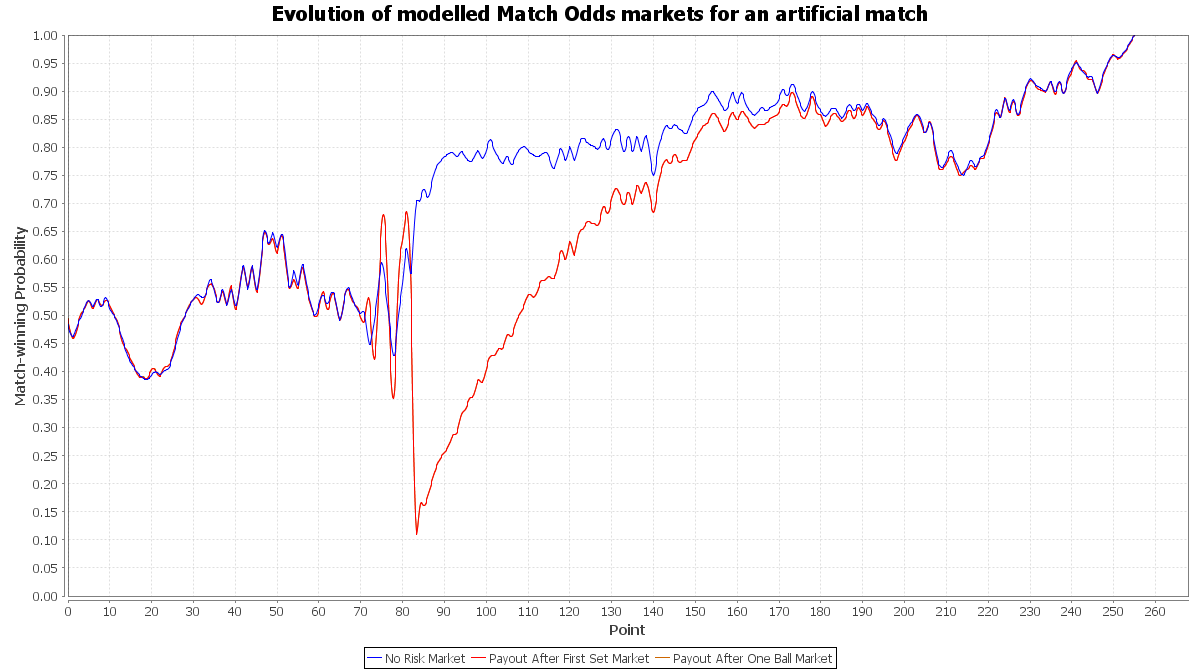
\includegraphics[width=12.5cm]{matches/artificialwin}
\caption{Evolution of Match Odds markets with a variety of retirement payout policies for an artificial match ($P_A = P_B = 0.6$, $c = 0.000115$, $\lambda = 10.0$, $\rho = 0.95$) with respect to Player A.  In this match, Player A receives an injury in the second set but rallies and continues on to victory}
\label{artificialwin}
\end{figure}

\begin{figure}[H]
\centering 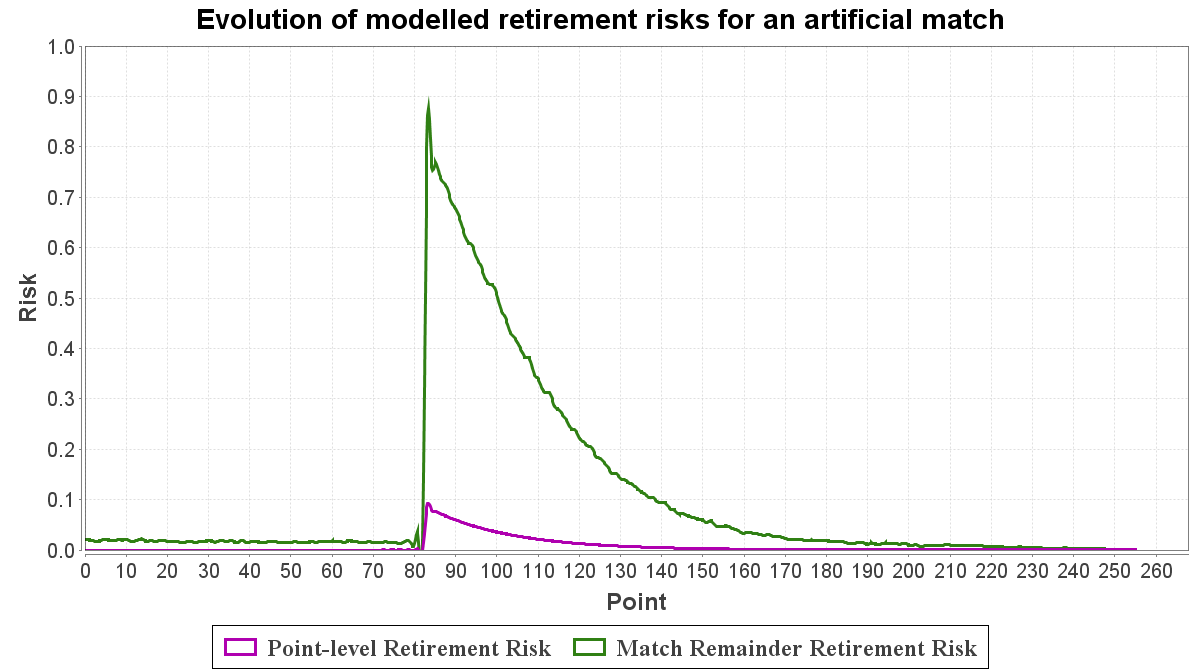
\includegraphics[width=12.5cm]{matches/artificialwinrisk}
\caption{Evolution of point-level and match-level retirement risks for an artificial match ($P_A = P_B = 0.6$, $c = 0.000115$, $\lambda = 10.0$, $\rho = 0.95$) with respect to Player A.  In this match, Player A receives an injury in the second set but rallies and continues on to victory}
\label{artificialwinrisk}
\end{figure}

\begin{figure}[H]
\centering 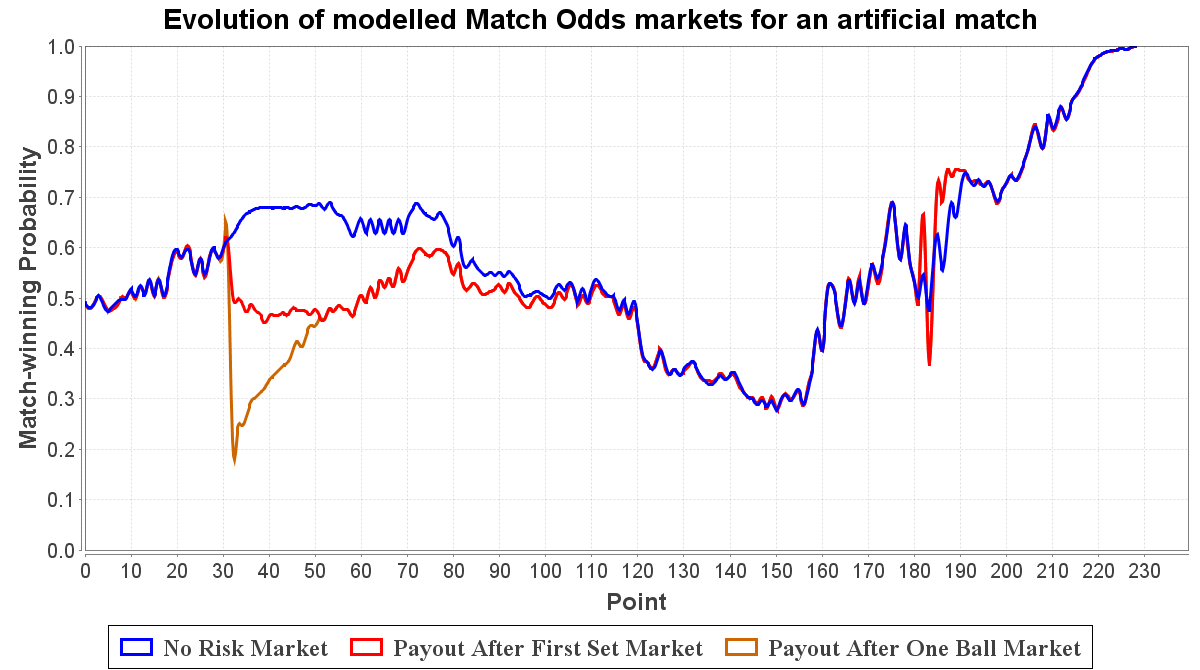
\includegraphics[width=12.5cm]{matches/artificialfirstset}
\caption{Evolution of Match Odds markets with a variety of retirement payout policies for an artificial match ($P_A = P_B = 0.6$, $c = 0.000115$, $\lambda = 10.0$, $\rho = 0.95$) with respect to Player A.  In this match, Player A receives an injury in the first set but rallies and continues on to victory}
\label{artificialfirstset}
\end{figure}

\begin{figure}[H]
\centering 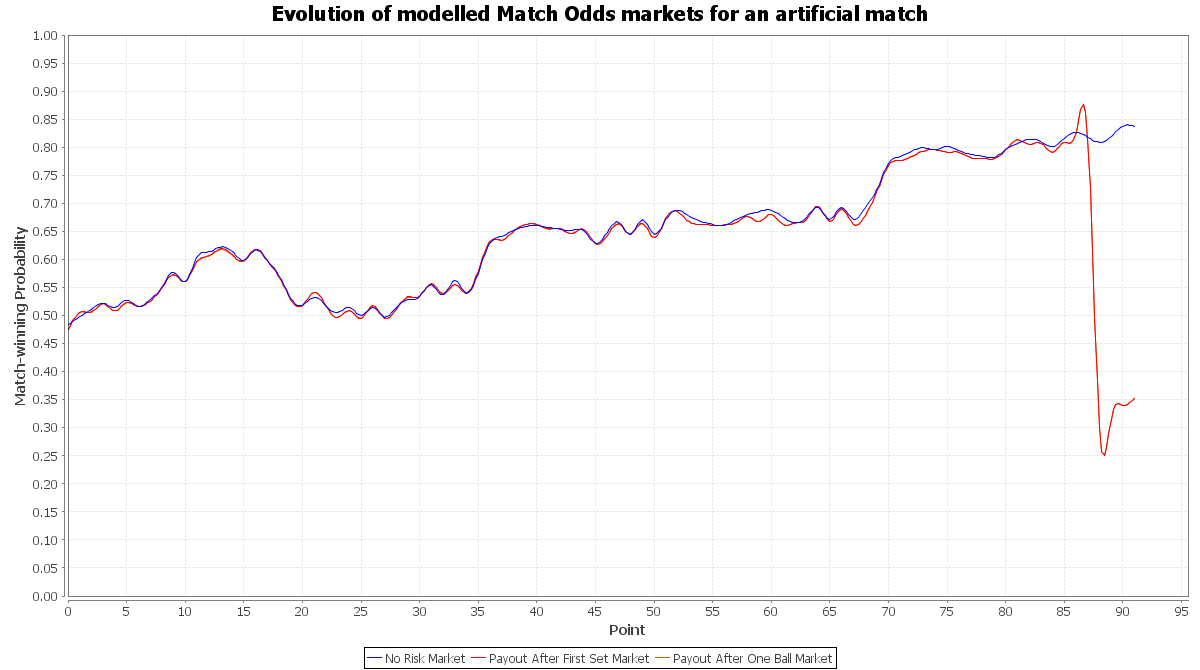
\includegraphics[width=12.5cm]{matches/artificialretirement}
\caption{Evolution of Match Odds markets with a variety of retirement payout policies for an artificial match ($P_A = P_B = 0.6$, $c = 0.000115$, $\lambda = 10.0$, $\rho = 0.95$) with respect to Player A.  In this match, Player A receives an injury and has to retire}
\label{artificialretirement}
\end{figure}

\subsection{Application to Real Data}

Our model appears to produce reasonable results from the beginning of a match given our assumption that players begin matches with no risk of retiring ($r_0^A = r_0^B = 0$).  Our model must also be applicable for any given match state, including the situation where an injury has recently occurred but the affected player is continuing to play.  At this stage, we know the gap in the odds for each player ($G_A$ and $G_B$), but how can we go \textit{backwards} from this and calculate the retirement risk for the \textit{current point}, $r_n^A$ and $r_n^B$ (which will naturally be a lot smaller)?  Once again, we can use the Nelder-Mead method to approximate these values for each point in the match.  Given this information, our simulator will be able to calculate the match-level retirement risk for each player at each point ($R_n^A$ and $R_n^B$).

Remember, we can imitate a Betfair-style \textit{after one set} payout policy market for Player A (and similarly for Player B) by computing:

\begin{center}
	$W_A^{''} = \frac{(W'_A + R_B^{''})}{(W'_A + R_B^{''}) + (W'_B + R_A^{''})}$
\end{center}

Now we are dealing with the gaps in the odds rather than the retirement risks to be output so we redefine our objective function as:

\begin{center}
	$\left|W_A - (W_A^{''} + G_A)\right| + \left|W_B - (W_B^{''} + G_B)\right|$
\end{center}

We now also have all the information we need to be able to predict the evolution of a market with an \textit{after one ball} payout policy for a real match using just the two Betfair markets!

\subsubsection{Preparing the Match Data}

Obtaining the Betfair odds data for a match was only the first step.  We also needed to acquire other match-specific information.  We needed to be able to read the current score into the model at any stage in the match.  We entered point-by-point data manually into CSV files using the archived point-level live scoring provided by website \textit{TennisEarth.com}\footnote{http://www.tennisearth.com} and tennis statistics software OnCourt\footnote{http://www.oncourt.info}.  

Up until this point, we have assumed that we will be able to manually input the point-winning probabilities on serve of both players in the match.  Due to \cite{dominance}, we know that the average point-winning probability on serve for a top-level professional tennis player, $\gamma$, is 0.645 for men and 0.560 for women.  We also have the insight, arising from \cite{omalley} and described by \cite{marek}, that the important thing in determining the winner of a match is the \textit{difference}, $\delta$, between the point-winning probabilities of each player and not the absolute values.  Consequently, if we can find what $\delta$ \textit{should} be, we can choose appropriate values for $P_A$ and $P_B$ by using the constraint that their average equals $\gamma$.  We must find both; we cannot, for example, fix $P_A$ to $\gamma$ and linearly search for $P_B$, since the model would cease to be symmetric for both players.  We know the current implied match-winning probability of the Set Betting (no retirement risk) market for both players and so we can do a simple binary search to find a value for $\delta$ (and therefore values for $P_A$ and $P_B$) for which O'Malley's tennis formulae generate the same results as the \textit{no risk} market.  Marek also states that for one to be able to express match-winning probability as a function of $\delta$, one must constrain $-0.1 \leq \delta \leq 0.1$.  Since the market's opinion of each player's point-winning probability changes throughout the match, we recalculate $P_A$ and $P_B$ on every point.  Note that this does not invalidate the assumption that points are iid as no dependency between points is introduced.

Another issue was how to match the odds data to the score at each point.  For instance, we may have many thousands of odds data lines for a match but only a couple of hundred points.  Although we have a timestamp for each line of odds data, we do not know the exact time that each point was played.  To overcome this challenge, we make the reasonable assumption that points happen at regular intervals.  For example, if we have 9000 lines of odds data for a match and 300 points were played, we would sample every $9000 / 300 = 30^{th}$ line.  Consequently, our modelled markets will appear more sparse than the original odds data as we only have as many points as there were points played in the match.

We now test our system on a number of real-world case studies.  We consider only the evolution of the in-play markets from the point of view of the player that was injured in the match (it is extremely rare that both players in a match receive significant injuries).

\section{Case Studies}

\subsection{Andy Murray vs Michael Berrer}

Figure \ref{murrayberrer2} displays processed Betfair odds data for the French Open 2011 third round match between Andy Murray and Michael Berrer that we discussed earlier.  In Figure \ref{murrayberrermodel}, we use our system to model Match Odds markets under three different retirement payout policies using the current score, estimated point-winning probabilities, and the positive gap created by subtracting the Betfair Match Odds implied probabilities on each point from the Betfair Set Betting probabilities, as input.  As you can see from the graph, our system reproduces the Betfair Match Odds market (red line) quite accurately with the \textit{after one set} modelled market.  This shows that we were successful in finding point-level retirement risks that would recreate the gap between the Betfair Set Betting and Match Odds markets.  The orange line shows our predicted \textit{after one ball} modelled market.  In this case, it closely follows the red \textit{after one set} market since the injury to Andy Murray occurs after the first set has been completed.

Bear in mind that there will always be a certain amount of variation due to the inexact nature of the simulator and our method of aligning our point-by-point data with the odds data.

\begin{figure}[H]
  \centering 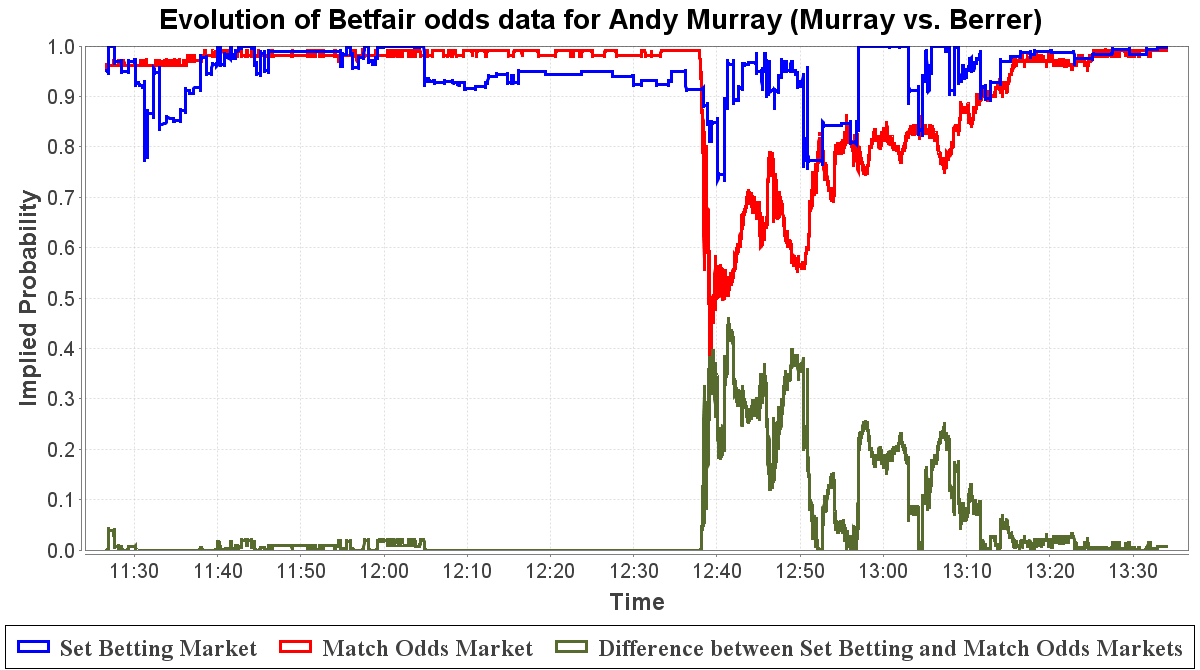
\includegraphics[width=12.3cm]{matches/murrayberrer}
  \caption{Evolution of implied match-winning probabilities extracted from the Betfair Match and Set Betting markets as well as the gap between them for Andy Murray - \textit{Murray vs. Berrer (French Open 2011 Men's Third Round)}}
  \label{murrayberrer2}
\end{figure}

\begin{figure}[H]
  \centering 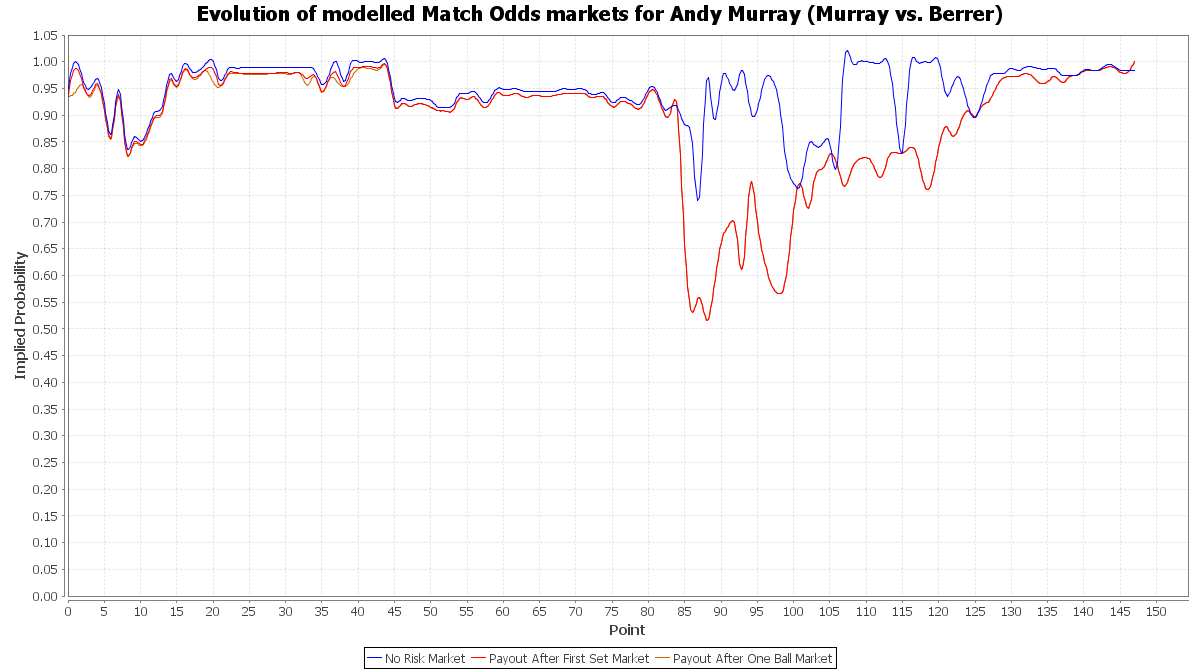
\includegraphics[width=12.3cm]{matches/murrayberrermodel}
  \caption{Evolution of modelled Match Odds markets under three different retirement payout policies for Andy Murray - \textit{Murray vs. Berrer (French Open 2011 Men's Third Round)}}
  \label{murrayberrermodel}
\end{figure}

\begin{figure}[H]
  \centering 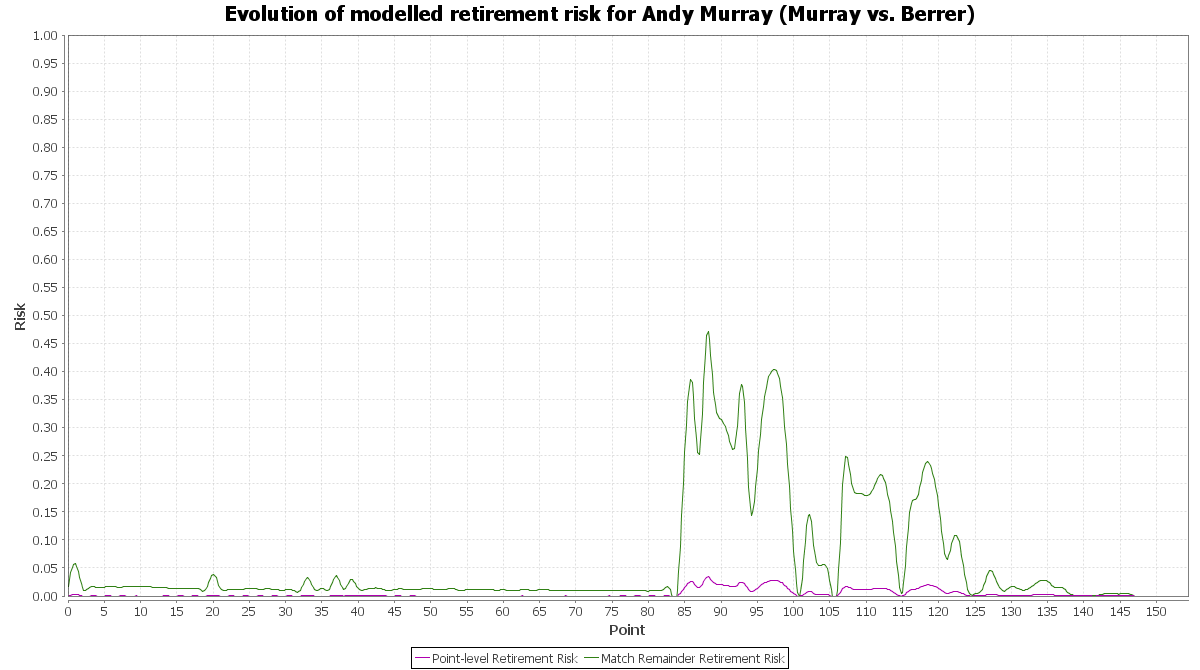
\includegraphics[width=12.3cm]{matches/murrayberrerrisk}
  \caption{Evolution of modelled point-level and remainder of match retirement risks for Andy Murray - \textit{Murray vs. Berrer (French Open 2011 Men's Third Round)}}
  \label{murrayberrerrisk}
\end{figure}

Figure \ref{murrayberrerrisk} shows the evolution of Andy Murray's risk of retirement throughout the match.  The green line follows the probability of retirement during the remainder of the match from the given point ($R_n$), whereas the magenta line gives the probability of retiring on a particular point itself ($r_n$).  Our model predicts a peak match-level retirement risk of 45\% during the injury period.  This coincides with a peak point-level retirement risk of 3\%.  Despite the severity of the injury, Murray's position of dominance in the match may be one explanation for why his risk of retirement is not greater. Berrer is still not expected to win the match irrespective of his opponent's misfortune.

\subsection{Rafael Nadal vs David Ferrer}

An all-Spanish Australian Open 2011 Men's Quarter Final saw Rafael Nadal battle veteran and fellow clay court specialist David Ferrer.  A mystery injury early on in the first set meant Nadal struggled throughout the match but he refused to retire and allowed his opponent the three-love win.

Figure \ref{nadalferrermodel} illustrates a scenario where an \textit{after one ball} modelled market can react differently than an \textit{after one set} market.  As we would expect (since the injury occurred in the first set), our predicted \textit{after one ball} market (orange line) anticipates an even greater drop in Nadal's match-winning probability around the time of his injury than the Betfair Match Odds \textit{after one set} market.  In the event of a Nadal retirement, such a market would pay out for a David Ferrer win as long as one ball has been played so at this point, traders would be very reluctant to back Nadal if he showed signs he might retire.  As the match moves past the first set, the \textit{after one ball} and \textit{after first set} lines merge since potential injuries now contribute to both markets equally.

\begin{figure}[H]
  \centering 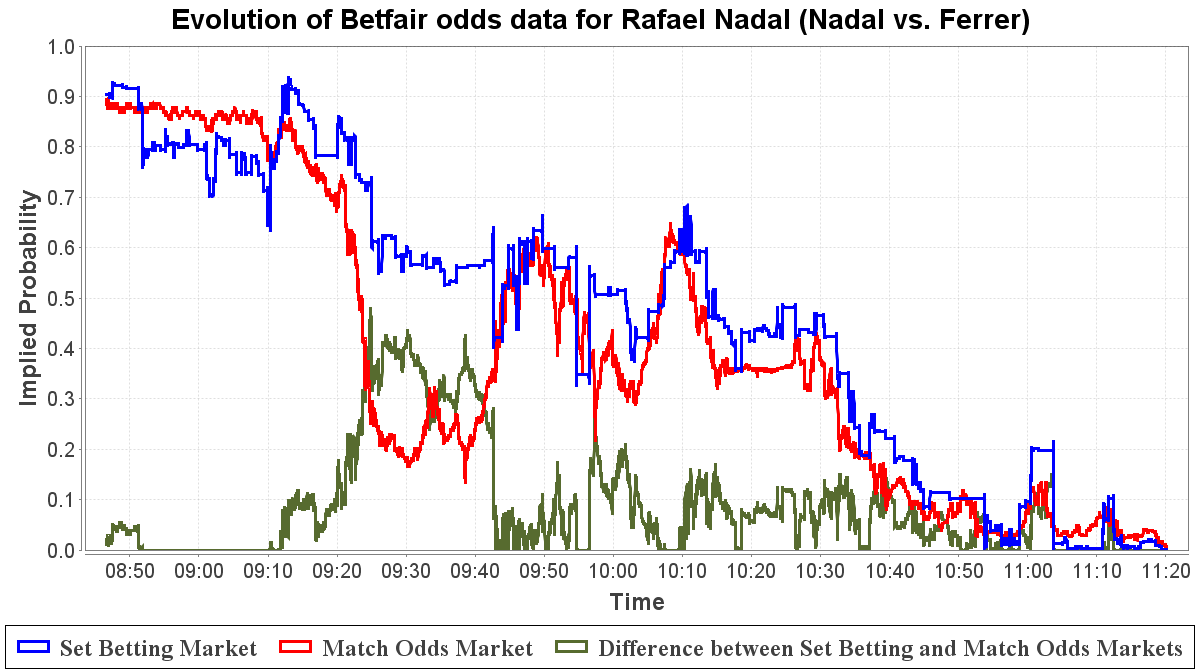
\includegraphics[width=12.3cm]{matches/nadalferrer}
  \caption{Evolution of implied match-winning probabilities extracted from the Betfair Match and Set Betting markets as well as the gap between them for Rafael Nadal - \textit{Nadal vs. Ferrer (Australian Open 2011 Men's Quarter Final)}}
  \label{nadalferrer}
\end{figure}

\begin{figure}[H]
  \centering 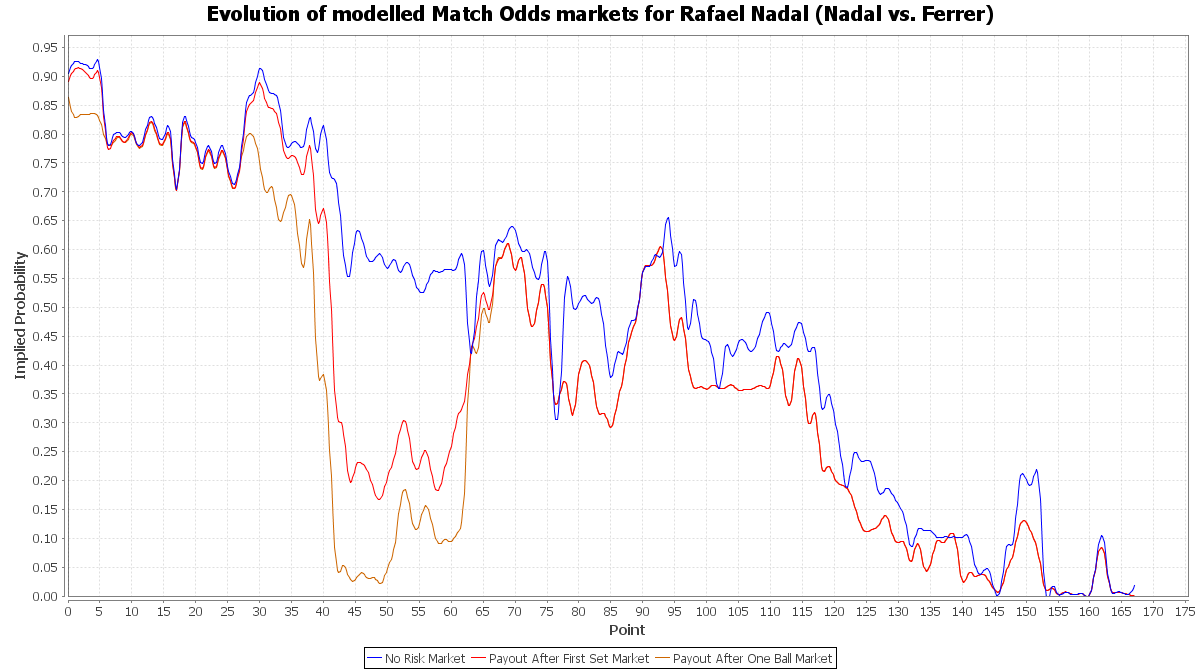
\includegraphics[width=12.3cm]{matches/nadalferrermodel}
  \caption{Evolution of modelled Match Odds markets under three different retirement payout policies for Rafael Nadal - \textit{Nadal vs. Ferrer (Australian Open 2011 Men's Quarter Final)}}
  \label{nadalferrermodel}
\end{figure}

\begin{figure}[H]
  \centering 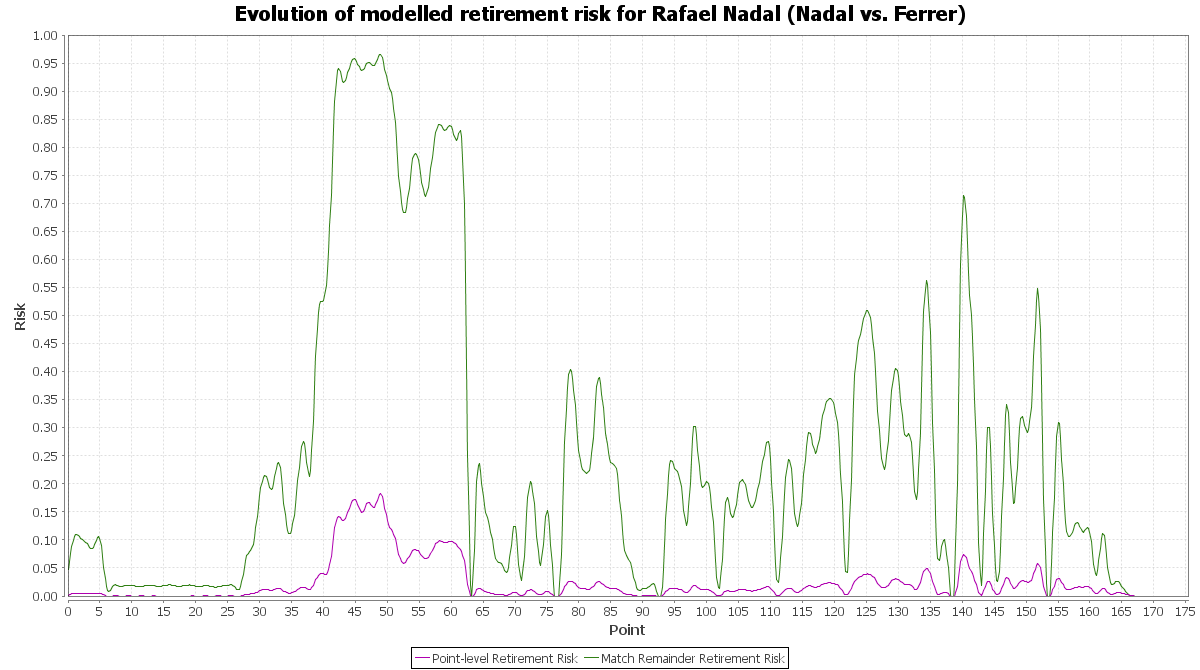
\includegraphics[width=12.3cm]{matches/nadalferrerrisk}
  \caption{Evolution of modelled point-level and remainder of match retirement risks for Rafael Nadal - \textit{Nadal vs. Ferrer (Australian Open 2011 Men's Quarter Final)}}
  \label{nadalferrerrisk}
\end{figure}

Figure \ref{nadalferrerrisk} shows the evolution of Rafael Nadal's risk of retirement throughout the match.  Our model predicts a high peak match-level retirement risk of 96\% during the injury period.  This coincides with a peak point-level retirement risk of 18\%.

As the match progresses and Nadal falls further behind, we see spikes in his retirement risk despite there being no large gaps between the Betfair markets.  This happens when the Match Odds market gives a player little chance of winning the match.  We illustrate how this occurs with an example.  Say that on a particular point, the Set Betting market tells us that the implied probability of Nadal winning the match is 0.5.  This means that we can assign $P_A = P_B = 0.645$.  We also happen to know that the difference between the Betfair Set Betting and Match Odds markets for Nadal is 0.4.  We now look for a value of $r_A$ (retirement risk of Nadal on this point) such that $W_A^{''}$ (probability of winning the match normally with retirement risk after the first set only) is only 0.1.  Since we have $P_A = P_B$ and therefore both players have an equal chance of winning the match if it does not end in retirement, we have $W_B^{''} = 0.1$ and so the sum of the probabilities of either player winning the match normally is only 0.2.  Making the assumption that $r_n^B$ is negligible, we must have that $R_A \approx 0.8$ (retirement risk of Nadal in the match).  This can happen in any situation where $W^{''}$ is small and there is a risk of retirement, like towards the end of this quarter final.

Such scenarios, as well as our choice of matches where only one player was injured, help to explain why our predicted retirement risk is generally much larger than the gap in the Betfair markets.

\subsection{Victoria Azarenka vs. Maria Sharapova}

Victoria Azarenka faced off against Maria Sharapova in the Rome Masters 2011 Quarter Final.  Unfortunately, Azarenka suffered a hand injury early in the second set while leading one set to love and was unable to continue the match.

As you can see in Figure \ref{azarenkasharapovarisk}, we have spikes of retirement risk during the first set which correspond with sporadic drops in the implied probability of our predicted \textit{after one ball} market.  These anomalies appear to coincide correctly with small gaps created where the \textit{after one set} market model is beneath the Set Betting market.  However, the tiniest of these gaps can correspond to a significant drop in the implied probability of \textit{after one ball} market.  Whenever we have such a gap, we attempt to find a point-level probability ($r_n$) that will recreate this gap.  Since the Betfair Match Odds market only takes into account retirement after the first set, only retirements after the first set can affect our model of this market.  However, the system has no direct control over retirements \textit{after} the first set if we are still in the first set.  The more you try to increase the immediate point-level retirement risk, the more likely the given player will retire straight away (still in the first set).  Lower it so the player will survive past the first set and he or she probably will not retire.  The consequence of this is that our \textit{after one ball} market model (and therefore our predicted retirement risk) is very sensitive to the Betfair odds source data, particularly towards the beginning of the first set.

Nonetheless, this match is still a good example of how unpredictable injury occurrence is.  Azarenka's match-level retirement risk still stays relatively low until the injury occurs on point 75.  The risk shoots up to 54\%, peaking at 89\% at retirement on point 93 after a brief dalliance with the possibility of recovery.

\begin{figure}[H]
  \centering 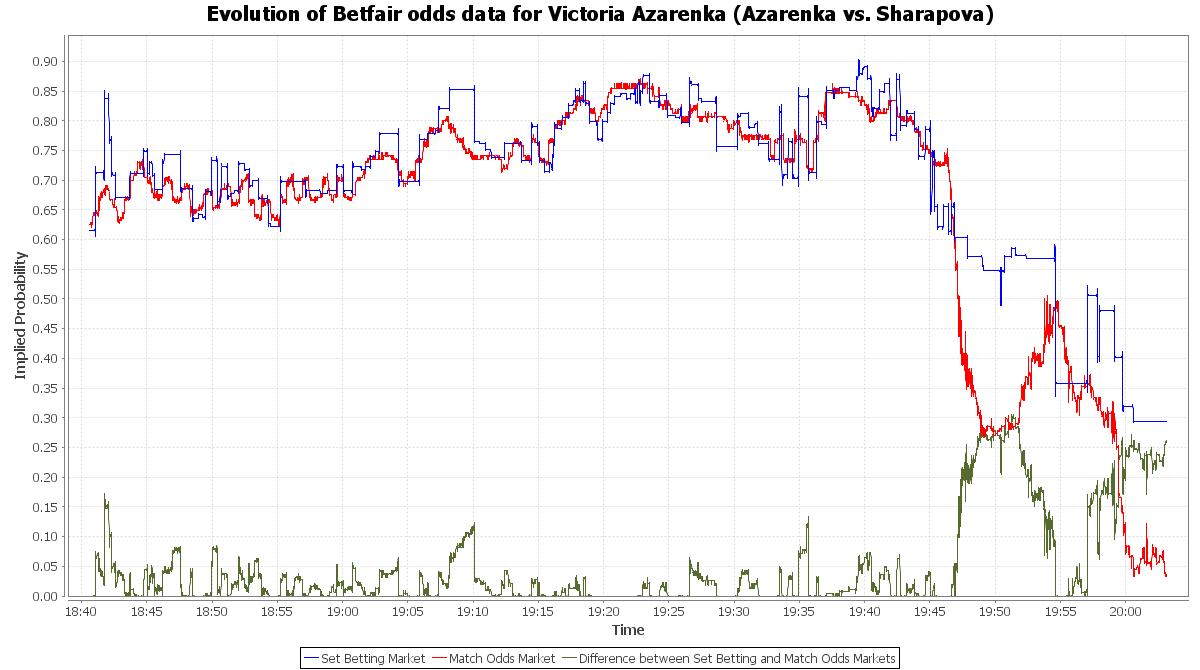
\includegraphics[width=12.3cm]{matches/azarenkasharapova}
  \caption{Evolution of implied match-winning probabilities extracted from the Betfair Match and Set Betting markets as well as the gap between them for Victoria Azarenka - \textit{Azarenka vs. Sharapova (Rome Masters 2011 Women's Quarter Final)} [ended in retirement]}
  \label{azarenkasharapova}
\end{figure}

\begin{figure}[H]
  \centering 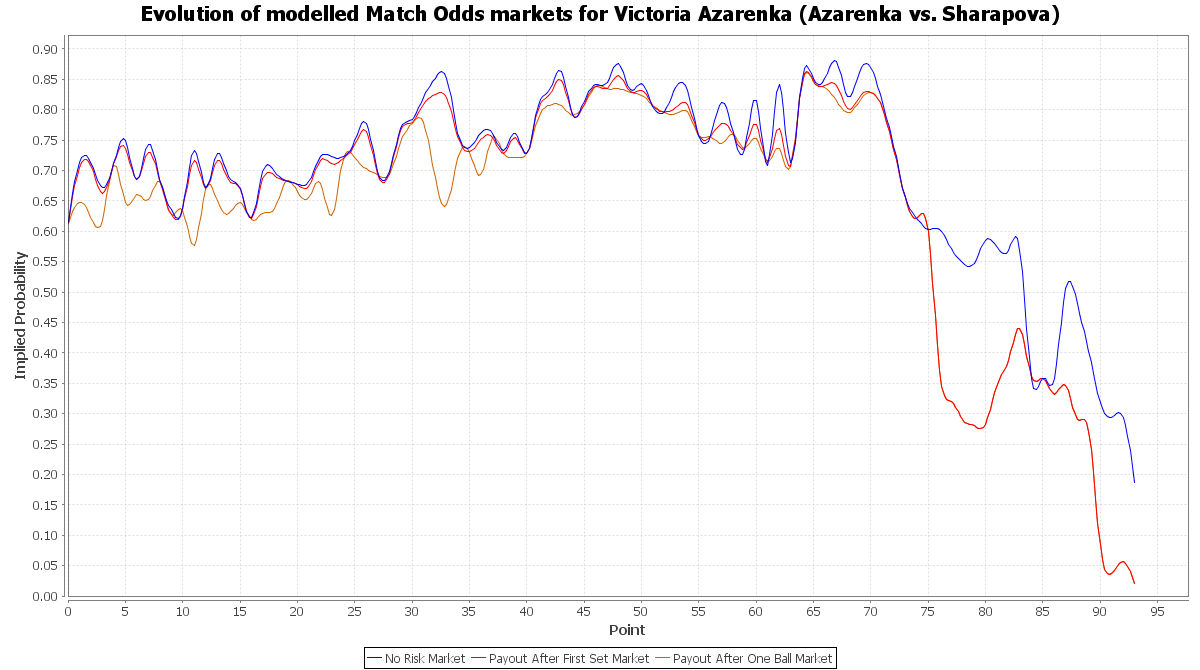
\includegraphics[width=12.3cm]{matches/azarenkasharapovamodel}
  \caption{Evolution of modelled Match Odds markets under three different retirement payout policies for Victoria Azarenka - \textit{Azarenka vs. Sharapova (Rome Masters 2011 Women's Quarter Final)} [ended in retirement]}
  \label{azarenkasharapovamodel}
\end{figure}

\begin{figure}[H]
  \centering 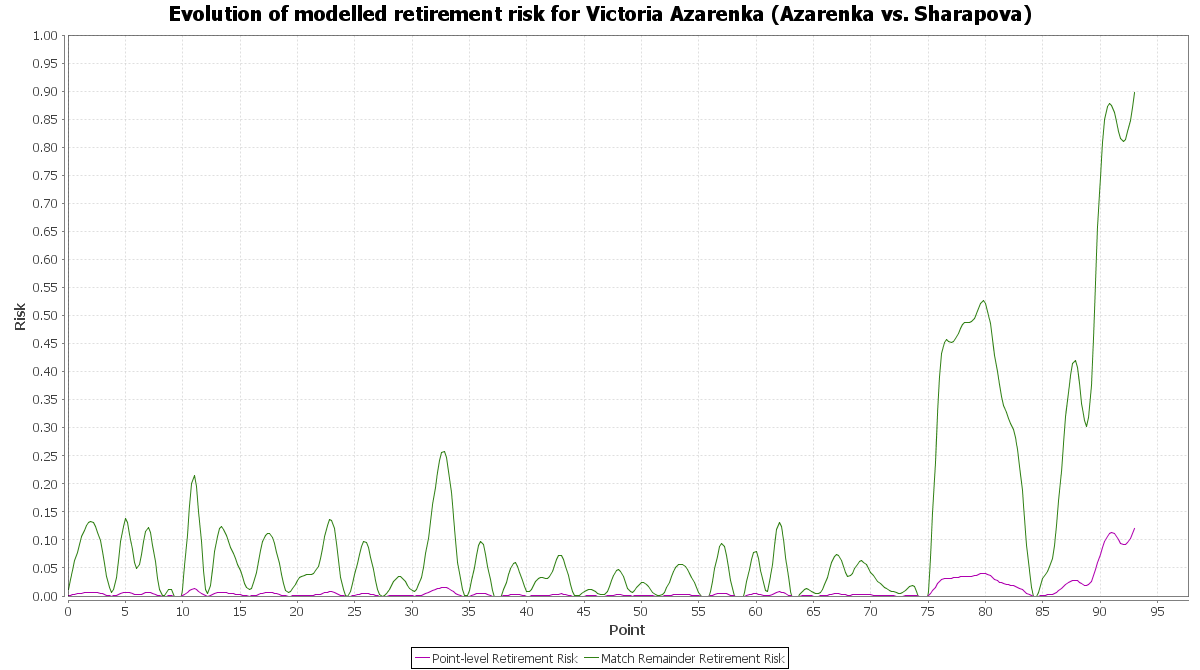
\includegraphics[width=12.3cm]{matches/azarenkasharapovarisk}
  \caption{Evolution of modelled point-level and remainder of match retirement risks for Victoria Azarenka - \textit{Azarenka vs. Sharapova (Rome Masters 2011 Women's Quarter Final)} [ended in retirement]}
  \label{azarenkasharapovarisk}
\end{figure}

\section{Conclusions}

We confirm that it is possible to observe the occurrence of an injury in a given tennis match by observing the evolution of the in-play betting odds.  We examine historical Betfair odds for a number of real-life matches and find that a gap between markets that use different player retirement payout policies is created in correspondence with the occurrence of an injury in the match.  We note that injuries have a drastic effect on the odds data, in many occasions turning the overwhelming favourite into the underdog in an instant.

We have created a new model for retirement risk in tennis matches and implemented it into a tennis match simulator by incorporating extra parameters approximated using real-world averages and betting odds data as well as additional match outcomes compared to standard tennis models.  To the best of our knowledge, this is the world's first published attempt to create such a model.  Testing the model in a completely artificial environment, we found it was able to mimic the expected patterns of in-play betting markets with different retirement payout policies for matches with varying injury scenarios.

We conclude that a given player's risk of retirement at some point during the remainder of a match is a function of the difference between the odds of a Match Odds market for that player that ignores risk of retirement and the odds of a Match Odds market for that player that takes into account risk of retirement, for any given point in the match.  Our system provides a value for the retirement risk of a given player at any point in a match.

We applied our model to a number of real-world matches (from the point of view of an injured player) using Betfair odds data and produced imitations of the in-play betting markets following different player retirement payout rules.  We find that we can mimic to a good degree of accuracy the progress of the Betfair Set Betting and Match Odds in-play markets throughout matches, i.e. a \textit{match-completed} market and an \textit{after first set} market, respectively.  We attempt to use the Betfair odds data to predict the evolution of an \textit{after one ball} market.  We find that such a market generally correctly produces slightly lower match-winning implied probabilities than the Betfair Match Odds market when the given match is still in the first set, although it can be somewhat erratic.  The retirement risk values are very sensitive to any gap between the Betfair markets due to the lack of control our system has over retirement risk \textit{after} the first set when the match is still in the first set.  Furthermore, we notice that the system generates retirement risk spikes when the player in question has a low match-winning probability.  The problem underlying these fragilities in our predictions is that the Betfair in-play tennis betting markets are not perfect.  Since this odds data is vital input for our system, it is no surprise that fluctuating, anomalous, and sparse data heavily influences the output of our system.

We note that a potentially useful application of our model is in the real-time estimates of player retirement risk during professional tennis matches.  Such information could be displayed on-screen for the viewer during a live broadcast or used as a commentary aid.

% BibTeX support
\bibliographystyle{DeGruyter}
\bibliography{paper}

\end{document}